\chapter{Measurement Campaign}
\section{Setup}
The setup of the measurement will give the insight and solutions to the problems hypothesised in previous chapters. 

\begin{figure}[H]
\centering
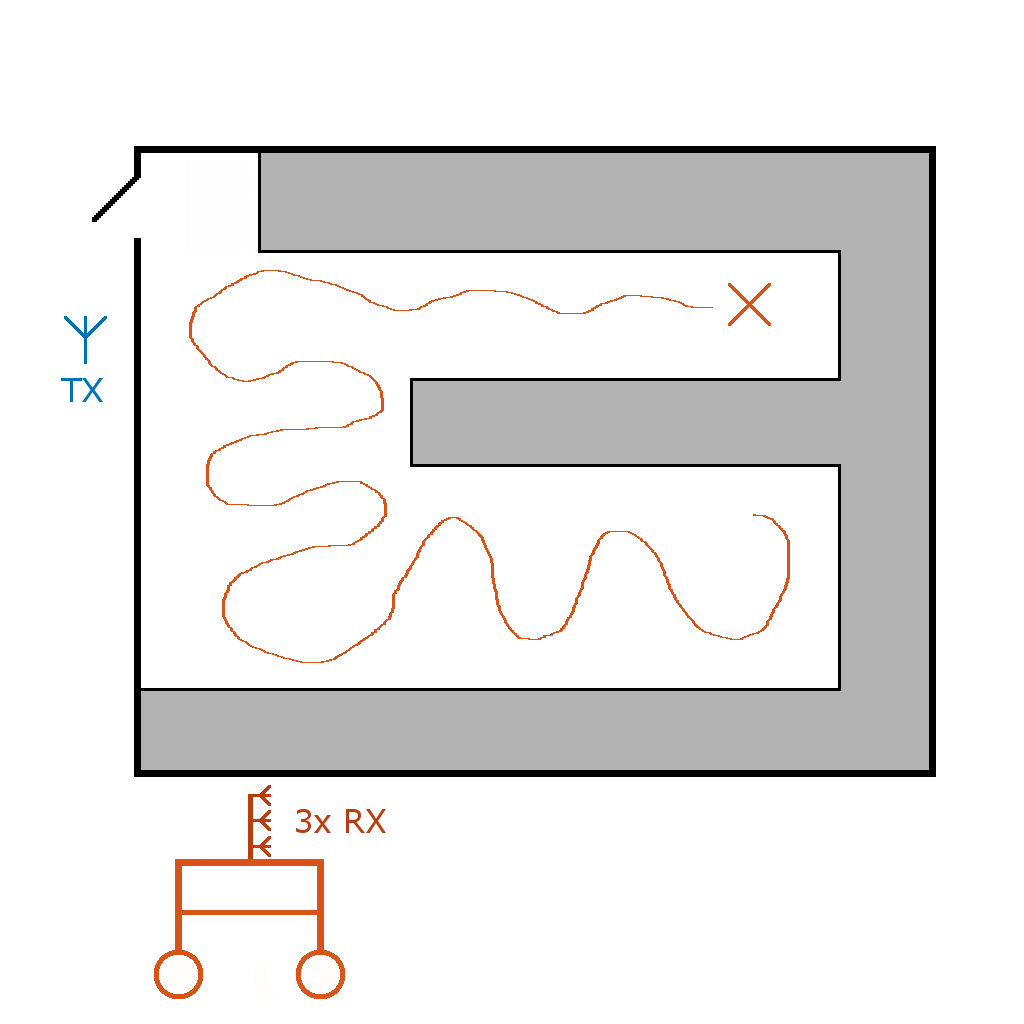
\includegraphics[width=0.75\textwidth]{figures/Gimp_figures/MeasSetup.png}
\caption{Sketch of the room}
\label{room sketch}
\end{figure}
\subsection{equipment}
\label{equip}
Keysight PNA N5527A 
10 Hz $IF_{bw} = -119dB$ Dynamic range.

Antenna array 4Ghz $f_c$.


%The most important part of the setup is the equipment and how they are connected. The R\&S Spectrum Analyser (model FPL9KHz-6GHz) is the center of the setup. This is the receiver of our system and gives us a readout of the spectrum in terms of power (dBm) and frequency (Hz). The two main setting on the Spectrum analyser is IF filter bandwidth and resolution. These two values gives us a sweep time.
\subsection{Specifications}
In chapter 1 all the needed factors has been discussed. Now when the setup is designed it's important to set specifications.
\begin{table}[]
\centering
\caption{My caption}
\label{final_specs}
\begin{tabular}{|l|l|l|l|}
\hline
Number of samples needed         & N           & 4.04 million   & $4.04 10^6$        \\ \hline
Center Frequency                 & $f_c$       & 4Ghz           & $4 \cdot 10^9$     \\ \hline
Wavelength                       & $\lambda$   & 10cm           & 0.075m               \\ \hline
Coherence freq                   & $\Delta f$  & 3MHz           & $3 \cdot 10^6$     \\ \hline
Dynamic range                    & DR          & 98dB           & $2\cdot 10^10$             \\ \hline
Antenna diversity                & $A_{div}$   & 1x3            & 3                  \\ \hline
Intermediate frequency bandwidth & $IF_{BW}$     & 10KHz          & $10 \cdot 10^3$ \\ \hline
\end{tabular}
\end{table}
\subsection{Total Dynamic range}
Given \autoref{total_prx} and the VNA specification given in \autoref{equip} we can find the total received power seen in the measurements and calculate the total dynamic range needed given the margin in \autoref{SNR_margin}:
\begin{equation}
L = 20log (4000MHz) + 28 \cdot log(5)-28 = 63.61dB \approx 64dB
\end{equation}
\begin{equation}
DR_{tot} = 64dB - 30dBm + 64dB = 98dB 
\end{equation}
We assume that the noise floor of the \gls{VNA} scales linearly with a increased $IF_{BW}$. This would mean that a $IF_{BW}$ on the \gls{VNA} can be increased by:
\begin{equation}
\begin{split}
&= IF_{BW} = 119dB-98dB = 21dB \\
           &= 10Hz \rightarrow 1kHz
\end{split}
\end{equation}
\section{Results}